
\documentclass[pdf]{beamer}

\usepackage{amsmath}
\usepackage{amssymb}
\usepackage{amsthm}
\usepackage{mathtools}

\usetheme{Dresden}
\usecolortheme{beaver}

%Analysis
\newcommand{\Rl}{\mathbb{R}}
\newcommand{\Cplx}{\mathbb{C}}
\newcommand{\Itgr}{\mathbb{Z}}
\newcommand{\Ntrl}{\mathbb{N}}
\newcommand{\Ind}{\mathbbm{1}}
\newcommand{\Hlbt}{\mathcal{H}}
\newcommand{\im}{\operatorname{im}}

%Algebra
\newcommand{\Grp}{\mathcal{G}}

%Misc
\newcommand{\lra}{\longrightarrow}
\newcommand{\ra}{\rightarrow}
\newcommand{\lla}{\longleftarrow}
\newcommand{\la}{\leftarrow}

%Stats \ Prob
\newcommand{\E}[1]{\mathbb{E} \left[ #1 \right]}
\newcommand{\Var}[1]{\operatorname{Var} \left[ #1 \right] }
\newcommand{\Cov}[2]{\operatorname{Cov} \left[ #1, #2 \right] }
\newcommand{\Filt}{\mathcal{F}}

%Fractional Differential Equations

\newcommand{\laplace}[1]{ \mathcal{L} \left\{ #1 \right\} }
\newcommand{\fourier}[1]{ \mathcal{F} \left\{ #1 \right\} }
\newcommand{\mellin}[1]{ \mathcal{M} \left\{ #1 \right\} }
\newcommand{\rld}[3]{ \left( \mathcal{D}_{#1}^{#2} #3 \right) }
\newcommand{\rli}[3]{ \left( I_{#1}^{#2} #3 \right) }
\newcommand{\der}[3]{ \frac{d^{#3}#1}{d#2^{#3}} }
\newcommand{\capder}[3]{ \left( \prescript{C}{}{\mathcal{D}_{#1}^{#2}} #3 \right) }

\mode<presentation>{}
\title{A Stochastic Approach to Fractional Diffusion}
\subtitle{help I'm trapped in a LaTeX compiler}
\author{Ed McDonald \& Adam Gray}
\institute{
	School of Mathematics and Statistics \\
	University of New South Wales
}

\begin{document}

\begin{frame}
	\titlepage
\end{frame}

\begin{frame}{Outline}
    \begin{itemize}
        \item Standard diffusion
        \item Super diffusion
        \item Sub diffusion
        \item Solving a fractional differential equation
    \end{itemize}
\end{frame}


\begin{frame}{Central Limit Theorem and Random Walks}
	\begin{block}{Random Walk}
	    Let $ X_1, \ldots X_n $ be a sequence of random variables,
	    then 
	    \begin{align}
	        S_n = \sum_{k=1}^n X_n 
	    \end{align}
	    represents the position after $ n $ steps.
	\end{block}
	If $ \mathbb{E}[X_i] = 0 $ and  $ \mathbb{E}[X_i^2] = 2 $ then the central limit theorem gives us that
	\begin{align}
	    \frac{S_n}{\sqrt{n}} \lra Z
	\end{align}
	\emph{weakly} as $ n \lra \infty $, where $ Z \sim \mathcal{N}(0,2) $
\end{frame}

\begin{frame}{Central Limit Theorem and Random Walks}
    We can extend this idea by introducing a scaling paramter $ \gamma $.
    \begin{align}
        S_{\lfloor \gamma t \rfloor} = \sum_{k=1}^{\lfloor \gamma t \rfloor} X_k.
    \end{align}
    $ \gamma $ has the effect of changing the \emph{timescale} that we are considering the process running over.
    
    We can calculate the characteristic function of 
    \begin{align}
       \frac{S_{\lfloor \gamma t \rfloor}}{\sqrt{\gamma }}.
    \end{align}
    By the convolution theorems we can say that it is
    \begin{align}
        \left( 1- \frac{k^2}{\gamma} + o(\gamma^{-1}) \right)^{\lfloor \gamma t \rfloor}
    \end{align}
\end{frame}

\begin{frame}{Long Time Limit}
    We can rearrange
    \begin{align}
        \left( 1- \frac{k^2}{\gamma} + o(\gamma^{-1}) \right)^{\lfloor \gamma t \rfloor}
        &= \left[ \left( 1- \frac{k^2}{\gamma} + o(\gamma^{-1}) \right)^\gamma \right]^\frac{{\lfloor \gamma t \rfloor}}{\gamma}
    \end{align}
    and then take $ \gamma \lra \infty $ to get that
    \begin{align}
    \left[ \underbrace{\left( 1- \frac{k^2}{\gamma} + o(\gamma^{-1}) \right)^\gamma}_{\circledast} \right]^\frac{{\lfloor \gamma t \rfloor}}{\gamma} \lra e^{-tk^2}
    \end{align}
    by using the well known result
    \begin{align}
        \lim_{n \lra \infty} \left(1 + \frac{x}{n}\right)^n = e^x.
    \end{align}
\end{frame}


\begin{frame}{Fourier Transform and a PDE}
    Notice that $ e^{-tk^2} $ is just the CF of $Z_t \sim \mathcal{N}(0,2t) $. Further we can say that $ \frac{S_{\lfloor \gamma t \rfloor}}{\sqrt{\gamma}} \lra Z_t $ by LCT.
    
    
    We can also regard $ e^{-tk^2} $ as the FT of the density of $ Z_t $.
    
    Rather usefully we have also have that $ e^{-tk^2} $ is a solution to 
    \begin{align}
        \frac{d\hat{u}}{dt} = -k^2\hat{u}
    \end{align}
    
    We can actually use a analogous result from last week's homework to invert the Fourier transform of $ u $ to get
    \begin{align}
        \frac{\partial u}{dt} = \frac{\partial^2 u}{\partial x^2}
    \end{align}
\end{frame}

\begin{frame}{A More General Result}
    We can generalise this result a bit and say that if $ \mathbb{E}[X_i^2] = \sigma^2 $
    then $ \frac{S_{\lfloor \gamma t \rfloor}}{\sqrt{\gamma}} \lra Z_{t} $, but now $ Z_t \sim \mathcal{N}(0,2\sigma^2 t) $.
    
    Further the Fourier transform of the density of $ Z_t $ is $ e^{-t\sigma^2k^2} $
    which means the density is now a solution to
    \begin{align}
        \frac{\partial u}{\partial t} = \underbrace{\frac{\sigma^2}{2}}_{D}\frac{\partial^2 u}{\partial x^2}.
    \end{align}
    What this says is that as particles jump around more, they diffuse more rapidly.
\end{frame}


\begin{frame}{A Plot}
    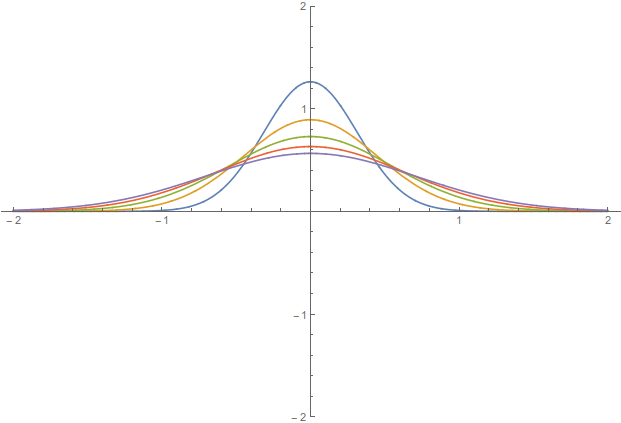
\includegraphics[scale=0.4]{Diffusion}
\end{frame}

\begin{frame}{Recap}
    \begin{itemize}
        \item All we have done to get this result is require that the random variables that represent the \emph{jumps} fullfill the requirements of the CLT.
        \item What if we relax the \emph{finite second moment} condition?
    \end{itemize}
\end{frame}
\begin{frame}{Pareto Distribution}
    \begin{itemize}
        \item Consider a random variable $ P $ with density $ Cx^{-\alpha-1} $ for some normalising constant $ C $.
        \item If we require $ 1 < \alpha < 2 $ then we have $ \mathbb{E}[P] $ exists but $ \mathbb{E}[P^2] = \infty $ does not.
        \item It can be shown (with very lengthy computation) that the FT of the density of $ P $ is $ 1 + (ik)^\alpha + O(k^2) $.
        \item The idea is to setup a sequence of random variables $ Y_1, \ldots Y_n $, all iid with Pareto distribution with parameter $ \alpha $ and use these as the \emph{jumps} in the random walk.
    \end{itemize}
    
\end{frame}

\begin{frame}{Pareto Distribution}
    Setup $ S_n = \sum_{k=1}^n Y_n $ as before.
    
    By the convolution theorems for FTs we can calculate the FT of the density of $ \frac{S_n}{n^\frac{1}{\alpha}} $ to be
    \begin{align}
        \left( 1 + \frac{(ik)^\alpha}{n} + O(n^{-\frac{2}{\alpha}}) \right)^n
    \end{align}
    Notice that as $ n \lra \infty $ this has limit $ e^{(ik)^\alpha} $.
    
    The LCT implies that $ \frac{S_n}{n^\frac{1}{\alpha}} \lra Z $ where $ Z $ has FT $ e^{(ik)^\alpha} $.
    
    Notice that in some way this is an \emph{Extended Central Limit Theorem}.
\end{frame}

\begin{frame}{Long Time Limit}
    Like before we can introduce a time scale paramter $ \gamma $ and write
    \begin{align}
        S_{\lfloor \gamma t \rfloor} = \sum_{k=1}^{\lfloor \gamma t \rfloor}Y_k.
    \end{align}
    Again by considering the FT of 
    \begin{align}
        \frac{S_{\lfloor \gamma t \rfloor}}{\gamma^\frac{1}{\alpha}}
    \end{align}
    which is
    \begin{align}
        \left( 1 + \frac{(ik)^\alpha}{\gamma} + o(\gamma^\frac{-2}{\alpha})\right)^{\lfloor \gamma t \rfloor}.
    \end{align}
\end{frame}

\begin{frame}{Long Time Limit}
    \begin{align}
            \left( 1 + \frac{(ik)^\alpha}{\gamma} + o(\gamma^\frac{-2}{\alpha})\right)^{\lfloor \gamma t \rfloor}
        \end{align}
        By taking $ \gamma \lra \infty $ we get that the Fourier transform converges to
        \begin{align}
            e^{t(ik)^\alpha}
        \end{align}
    and by the LCT this gives us that 
    \begin{align}
        \frac{S_{\lfloor \gamma t \rfloor}}{\gamma^\frac{1}{\alpha}} \lra Z_t
    \end{align}
    where $ Z_t $ has FT $ \hat{u}(k) = e^{t(ik)^\alpha} $.
    
    Notice that this is a stable distribution.
\end{frame}
\begin{frame}
    It is clear that $ \hat{u}(t) = e^{t(ik)^\alpha} $ is a solution to
    \begin{align}
        \frac{d\hat{u}}{dt} = (ik)^\alpha \hat{u}.
    \end{align}
    Unfortunately we can't use \emph{last week's homework} to invert this FT and this is where we introduce fractional calculus.
\end{frame}


\begin{frame}{Motivations}
	\begin{block}{Cauchy Formula for Repeated Integration}
		\begin{align*}
			\int_{a}^{x} \int_{a}^{y_1} \cdots \int_a^{y_{n-1}} f(y_n) dy_n \cdots dy_2 dy_1 = \frac{1}{(n-1)!} \int_a^x(x-t)^{n-1}f(t)dt
		\end{align*}
	\end{block}
	\pause
	The idea is to replace the factorials with gamma functions to define an integral of arbitrary order
	\pause
	\begin{block}{Riemann-Liouville Fractional Integral}
		\begin{align*}
			\rli{a}{\alpha}{f}(x) = \frac{1}{\Gamma(\alpha)} \int_a^x(x-t)^{\alpha-1}f(t)dt
		\end{align*}
	\end{block}
\end{frame}

\begin{frame}{Motivations (Derivatives)}
	\begin{block}{Riemann-Liouville Fractional Derivative}
		\begin{align*}
			\rld{a}{\alpha}{f}(x) &= \frac{d^{\lceil \alpha \rceil}}{dx^{\lceil \alpha \rceil}} \rli{a}{\lceil \alpha \rceil - \alpha}{f}(x) \\
				&= \frac{1}{\Gamma(1 - \alpha)}\frac{d^{n}}{dx^n} \int_a^x \frac{f(t)dt}{(x-t)^{\alpha - n + 1}}
		\end{align*}
		where $ n = \lfloor \alpha \rfloor + 1 $.
	\end{block}
\end{frame}

\begin{frame}{Motivations (Derivatives)}
	\begin{block}{Caputo Fractional Derivative}
		\begin{align*}
			\capder{a}{\alpha}{f}(x) &= \rli{a}{\lceil \alpha \rceil - \alpha}{\frac{d^{\lceil \alpha \rceil}}{dx^{\lceil \alpha \rceil}}f}(x) \\
				&= \frac{1}{\Gamma(1 - \alpha)} \int_a^x \frac{\frac{d^{t}}{dt^n}f(t)dt}{(x-t)^{\alpha - n + 1}}
		\end{align*}
		where $ n = \lfloor \alpha \rfloor + 1 $.
	\end{block}
\end{frame}
\begin{frame}{ Riemann-Liouville vs Caputo Derivative}
    \begin{itemize}
	\item The Caputo derivative is often used in fractional differential equations because it
	can be coupled with integer order initial conditions, whereas often the Riemann-Liouville
	derivative can't be coupled with integer order initial conditions.
   
    \item When we set $ a = -\infty $ for a large class of functions these derivatives are the same.
    \end{itemize}
\end{frame}

\begin{frame}{Fractional Derivative Fourier Transform}

	It can be shown that
	\begin{align}
	    \mathcal{F}\left\{\prescript{}{-\infty}{\mathcal{D}^\alpha}f(x) \right\} = (ik)^\alpha \mathcal{F}\{ f(x) \}
    \end{align}
    and it is precisely this result that we use to \emph{invert} the Fourier transform we had before.
    That is we can say that
    \begin{align}
        \frac{\partial u}{\partial t}(x,t) = \prescript{}{-\infty}{\mathcal{D}^\alpha_x} u(x,t)
    \end{align}
    where $u $ is the density of $ Z_t = \lim_{\gamma\lra\infty} \frac{Y_1 + Y_2 + \cdots + Y_{\lfloor \gamma t \rfloor}}{\gamma^\frac{1}{\alpha}} $.
    
    It can be shown that $ u(x,t) = Ax^{-\alpha-1} + o(x^{-\alpha-1}) $ as $ x \lra \infty $ with $ A $ depending on $ t $ and $ \alpha $.
\end{frame}

\begin{frame}{A Quick Note on the Laplace Transform}
	\begin{definition}
		We the define the Laplace transform of a function $ f $ to be the function $ F $
		given by
		\begin{align*}
			F(s) := \int_0^\infty e^{-st} f(t) dt
		\end{align*}
	\end{definition}
	
	We often write $ F(s) = \laplace{f(t)} $.
	
\end{frame}

\begin{frame}{A Quick Note on the Laplace Transform}
	
		
	
	The Laplace transform is particularly useful as it allows us to transform a differential equation into
	an ``algebraic'' equation. 
	
	Lerch's theorem guarantees, with minor caveats, that the Laplace transform of a function is
	unique.
	
\end{frame}

\begin{frame}{Basic Idea of the Laplace Transform Method}
	\begin{itemize}
		\item Apply the Laplace transform to both sides of the differential equation to get
		and "algebraic" equation.
		\item Apply the Laplace transform to the initial conditions. 
		\item Sub the transformed initial conditions into the transformed equation.
		\item Rearrange to get an expression for the Laplace transform of the function of interest.
		\item Invert. (This is possible, and guaranteed with minor caveats by Lerch's theorem)
	\end{itemize}
\end{frame}

\begin{frame}{The Laplace Transform of the Riemann-Liouville Integral}
	\begin{lemma}
	The Laplace transform of the Riemann-Liouville integral of a function $ f $ is given by
		$$ \mathcal{L} \left\{ I_0^\alpha f \right\}  = s^{-\alpha} \mathcal{L} \left\{ f \right\}.	$$
	\end{lemma}
\end{frame}

\begin{frame}{The Laplace Transform of the Riemann-Liouville Integral[Proof]}
	Since 
	$$
		 (I_0^\alpha f)(t) = \frac{1}{\Gamma(\alpha)} \int_0^t f(u) (t-u)^{\alpha - 1} du
	$$
	is just $ \frac{1}{\Gamma(\alpha)} $ times the convolution of $ f $ with $ t^{\alpha - 1} $ then by the convolution theorem
	for Laplace transforms we have that 
	\begin{align*}
		\mathcal{L} \left\{ I_0^\alpha f \right\} &= \frac{1}{\Gamma(\alpha)} \mathcal{L} \left\{ \int_{0}^{t} f(u) (t-u)^{\alpha - 1} du \right\} \\
			&= \frac{1}{\Gamma(\alpha)} \mathcal{L} \left\{ f(t) \right\} \underbrace{\mathcal{L} \left\{ t^{\alpha - 1} \right\}}_{=s^{-\alpha} \Gamma(\alpha)} \\
			&= s^{-\alpha} \mathcal{L} \left\{ f \right\}.
	\end{align*}
	\qed
\end{frame}

\begin{frame}{The Laplace Transform of the Caputo Derivative}
	The Laplace transform of the Caputo derivative of  a function $ f $ is given by
	\begin{align*}
		\laplace{\capder{0}{\alpha}{f}} = s^{\alpha - n} \left[ s^n \laplace{f} - \sum_{k=0}^{n-1} s^{n-k-1} \left( \der{f}{t}{k} \right)(0) \right].
	\end{align*}
\end{frame}

\begin{frame}{The Laplace Transform of the Caputo Derivative [Proof]}
	See that
	\begin{align*}
		\laplace{\capder{0}{\alpha}{f}} &= \laplace{  \rli{0}{n-\alpha}{\der{f}{t}{n}}} \\
			&= \underbrace{\frac{1}{\Gamma(n-\alpha)}\laplace{ \int_0^t (t-u)^{n-\alpha-1} \der{f}{t}{n} du}}_{\circledast} \\ 
	\end{align*}
\end{frame}

\begin{frame}{The Laplace Transform of the Caputo Derivative [Proof]}
	$ \circledast $ is just the Laplace transform of a convolution so 
	\begin{align*}
		\circledast &= \laplace{t^{n-\alpha-1}} \laplace{\der{f}{t}{n}} \\
		&= \frac{1}{n-\alpha} \left( s^{-(n-\alpha)} \Gamma(n-\alpha) \right) \\
		& \ \ \ \times \left( s^n \laplace{f} - \sum_{k=0}^{n-1} s^{n-k-1} \left( \der{f}{t}{k} \right)(0) \right) \\
		&= s^{\alpha - n} \left[ s^n \laplace{f} - \sum_{k=0}^{n-1} s^{n-k-1} \left( \der{f}{t}{k} \right)(0) \right].
	\end{align*}
	\qed
\end{frame}

\begin{frame}{One Parameter Mittag-Lefler Function}
	\begin{definition}
		The one parameter Mittag-Lefler $ E_\alpha $ function is defined by its power series.
		$$
			E_\alpha(t) = \sum_{k=0}^{\infty} \frac{t^k}{\Gamma(\alpha k + 1)}
		$$
	\end{definition}
\end{frame}

\begin{frame}{Laplace Transform of $E_\alpha(\beta t^\alpha)$}
	\begin{lemma}
		\begin{align*}	
			\laplace{ E_\alpha (\beta t^\alpha)} = \frac{s^{\alpha - 1}}{s^\alpha - \beta}
		\end{align*}
	\end{lemma}
\end{frame}

\begin{frame}{Laplace Transform of $E_\alpha(\beta t^\alpha)$ [Proof]}
See that
	\begin{align*}
		\laplace{ E_\alpha (\beta t^\alpha)} = \int_0^\infty e^{-st} \sum_{k=0}^\infty \frac{(\beta t^\alpha)^k}{\Gamma(\alpha k+1)} dt
	\end{align*}
	and because the series converges absolutely for all $ t \in \mathbb{R} $  we may interchange the integral
	and the sum to get
	\begin{align*}
		\int_0^\infty e^{-st} \sum_{k=0}^\infty \frac{(\beta t^\alpha)^k}{\Gamma(\alpha k+1)} dt &= \sum_{k=0}^\infty \int_0^\infty e^{-st} \frac{(\beta t^\alpha)^k}{\Gamma(\alpha k + 1)} dt \\
			&= \sum_0^\infty \frac{\beta^k}{\Gamma(\alpha k + 1)} \int_0^\infty e^{-st} t^{\alpha k} dt. \\
	\end{align*}
\end{frame}

\begin{frame}{Laplace Transform of $E_\alpha(\beta t^\alpha)$ [Proof]}
	By performing the change of variables $ x =st $ we get that 
	\begin{align*}
		\sum_0^\infty \frac{\beta^k}{\Gamma(\alpha k + 1)} \int_0^\infty e^{-st} t^{\alpha k} dt 
			&= \sum_0^\infty \frac{\beta^k s^{-(k+1)}}{\Gamma(\alpha k + 1)} \underbrace{\int_0^\infty e^{-x} x^{\alpha k} dx}_{\Gamma(\alpha k + 1)} \\
			&= \sum_{k=0}^\infty \beta^{k} s^{-(\alpha k + 1)} \\
			&= \frac{s^{\alpha-1}}{s^\alpha - \beta}.	
	\end{align*}
	\qed
\end{frame}

\begin{frame}{Summary of Important Results}
	\begin{align*}
		\laplace{\capder{0}{\alpha}{f}} &= s^{\alpha - n} \left[ s^n \laplace{f} - \sum_{k=0}^{n-1} s^{n-k-1} \left( \der{f}{t}{k} \right)(0) \right] \\
		\laplace{ E_\alpha (\beta t^\alpha)} &= \frac{s^{\alpha - 1}}{s^\alpha - \beta}
	\end{align*}
\end{frame}



\begin{frame}{The Solution to the Differential Equation}
	\begin{lemma}
		The fractional differential equation,
		\begin{align}
			\label{eq:fde-1}
			\left( \prescript{C}{}{\mathcal{D}_0^\alpha}y \right)(t) = \beta y(t) 
		\end{align}

		along with the initial conditions 
		\begin{align}
			\label{eq:fde-1-ic}
			y^{(k)}(0) = 
			\begin{cases}
				1 & k = 0 \\
				0 & 1 \leq k \leq \lfloor \alpha \rfloor - 1  
			\end{cases}
		\end{align}
		has solution
		$ y(t) = E_\alpha \left( \beta t^\alpha \right) $
	\end{lemma}
\end{frame}

\begin{frame}{Proof of Proposed Solution}
	Taking the Laplace transform of both sides of \eqref{eq:fde-1} yields
	\begin{align*}
		\laplace{\capder{0}{\alpha}{y}} &= \beta \laplace{y} \\
		s^{-(n+\alpha)} \left[s^n \laplace{y} - \sum_{k=0}^{n-1} s^{n-k-1} y^{(k)}(0) \right] &= \beta \laplace{y}
	\end{align*}
\end{frame}

\begin{frame}{Proof of Proposed Solution}
	Then taking into account \eqref{eq:fde-1-ic} (the initial conditions) we get
	\begin{align*}
		s^{-(n+\alpha)} \left[s^n \laplace{y} - s^{n-1}\right] &= \beta \laplace{y}
	\end{align*}
	and so 
	\begin{align*}
		\laplace{y} = \frac{s^{\alpha-1}}{s^\alpha - \beta}.
	\end{align*}
\end{frame}

\begin{frame}{Proof of Proposed Solution}
	By by noticing that 
	$$
		\laplace{y} = \frac{s^{\alpha-1}}{s^\alpha - \beta}.
	$$
	is the Laplace transform of $ E_\alpha(\beta t^\alpha) $ we have that
	\begin{align*}
		y(t) = E_\alpha(\beta t^\alpha)
	\end{align*}
	\qed
\end{frame}


	


\end{document}
